
\documentclass{beamer}
  \mode<presentation> {
    \usetheme{Frankfurt}
  }

\usepackage{times}
\usepackage{amsmath,amssymb}
\usepackage[english]{babel}
\usepackage[utf8]{inputenc}
% \usepackage[latin1]{inputenc}
\usepackage{array}
% % !BIB TS-program = biber
% !BIB program = biber
%===============================================================================
%          File: preamble.tex
%        Author: Pedro Ferrari
%       Created: 08 Feb 2017
% Last Modified: 08 Feb 2017
%   Description: Preamble for Thesis File
%===============================================================================
%---------------------------------------+
% Source code, programming and patching |
%---------------------------------------+
\usepackage{etoolbox}    % Toolbox of programming tools
\usepackage{xpatch}      % Extension of etoolbox patching commands

%--------------------------------------+
% Language, hyphenation, encoding, etc |
%--------------------------------------+
\usepackage[english]{babel}
\usepackage{lmodern}             % Use Latin Modern fonts
\usepackage[T1]{fontenc}         % Better output when a diacritic/accent is used
\usepackage[utf8]{inputenc}      % Allows to input accented characters
\usepackage{textcomp}            % Avoid conflicts with siunitx and microtype
\usepackage{microtype}           % Improves justification and typography
\usepackage[svgnames]{xcolor}    % Svgnames option loads navy (blue) colour

%---------------------------------------------+
% Page style: titles, margins, footnotes, etc |
%---------------------------------------------+
% A4 page layout:
\usepackage[width=14cm,left=3.5cm,marginparwidth=3cm,marginparsep=0.35cm,
height=21cm,top=3.7cm,headsep=1cm,footskip=1.1cm]{geometry}

\usepackage[pagestyles,outermarks]{titlesec}  % Customize titles and headers
\newpagestyle{main}[\scshape]{%
  \headrule
  \sethead
  [\thepage][][\chaptertitlename\space\thechapter. \chaptertitle]
  {\ifthesection{\thesection\space\,\sectiontitle}
  {\chaptertitlename\space\thechapter. \chaptertitle}}{}{\thepage}
}
\newpagestyle{special}[\scshape]{%
  \headrule
  \sethead
  [\thepage][][\chaptertitle]
  {\ifthesection{\sectiontitle}{\chaptertitle}}{}{\thepage}
}
% The following pagestyle is needed because titlesec isn't compatible with
% refsegment=chapter
\newpagestyle{bibatend}[\scshape]{
  \headrule
  \sethead
  [\thepage][][\chaptertitle]
  {\sectiontitle}{}{\thepage}
}
\pagestyle{special}
\appto{\mainmatter}{\pagestyle{main}}
\appto{\backmatter}{\pagestyle{bibatend}}
\appto{\printindex}{\pagestyle{special}}

% Use empty page style instead of plain in parts and chapters title pages
\patchcmd{\part}{plain}{empty}{}{}
\patchcmd{\chapter}{plain}{empty}{}{}

\usepackage{emptypage}  % Empty blank pages created by \cleardoublepage

% Change chapter heading style to match titlepage
\titleformat{\chapter}[display]
{\bfseries\filcenter}
{\titlerule[1.5pt]\vspace{4ex}%
\LARGE{\chaptertitlename\space\thechapter}}{0.5cm}{\huge}
[\vspace{2ex}{\titlerule[1.5pt]}\vspace{0.3cm}]
% Do the same for unnumbered chapters (TOC, preface, etc)
\titleformat{name=\chapter,numberless}[display]
{\bfseries\filcenter}
{\titlerule[1.5pt]\vspace{4ex}}{0.5cm}{\huge}
[\vspace{2ex}{\titlerule[1.5pt]}\vspace{0.3cm}]

\usepackage[stable,multiple]{footmisc}  % Customizations of footnotes
\renewcommand*{\footnoterule}{\vspace*{0.3cm}\hrule width 2.5cm\vspace*{0.3cm}}
\makeatletter
  \renewcommand\@makefntext[1]{
  \setlength{\parindent}{15pt}\mbox{\@thefnmark.\space}{#1}}
\makeatother

%-------------------------------+
% Math symbols and environments |
%-------------------------------+
\usepackage{amsmath}               % Load new math environments
\numberwithin{equation}{section}
\usepackage{amssymb}               % Defines most math symbols (such as \mathbb)
\usepackage{mathtools}             % Extension and bug fixes for amsmath package
\usepackage{mathrsfs}              % Math script like font
\usepackage{breqn}                 % Automatic line breaking of math expressions
\renewcommand*{\intlimits}{\displaylimits}  % Fix breqn clash with intlimits


%---------------------+
% Floats and captions |
%---------------------+
\usepackage{graphicx}           % To include graphics files
%\graphicspath{{/Users/Pedro/OneDrive/programming/Latex/logos/}{figures/}{tables/}}
\usepackage{pdflscape}
\usepackage[font=small,labelfont=bf]{caption}
\captionsetup*[figure]{format=plain,justification=centerlast,labelsep=quad}
\captionsetup*[table]{justification=centering,labelsep=newline}
\numberwithin{figure}{section}
\numberwithin{table}{section}

% Use subcaption for subfigures (to work properly with hyperref)
\usepackage{subcaption}
\captionsetup*[subfigure]{subrefformat=simple,labelformat=simple}
\renewcommand*{\thesubfigure}{(\alph{subfigure})}

% Further modifications of float layout
\usepackage[captionskip=5pt]{floatrow}  % We set caption skip here
\floatsetup[table]{style=Plaintop,font=small,footnoterule=none,footskip=2.5pt}

%----------------+
% Table packages |
%----------------+
\usepackage{array}          % Flexible column formatting
% \usepackage{spreadtab}  % Spreadsheet features
\usepackage{multirow}       % Allows table cells that span more than one row
\usepackage{booktabs}       % Enhance quality of tables
\setlength{\heavyrulewidth}{1pt}

% \usepackage{longtable}        % Allows to break tables through pages
% \floatsetup[longtable]{margins=centering,LTcapwidth=table}


%---------------------------------------------------------+
% Miscellaneous packages: lists, setspace, todonotes, etc |
%---------------------------------------------------------+
\usepackage[shortlabels,inline]{enumitem}   % Customize lists
\setlist[itemize,1]{label=$\bullet$}
\setlist[itemize,2]{label=\footnotesize{$\blacktriangleright$}}
\setlist[itemize,3]{label=\tiny{$\blacksquare$}}
\setlist[itemize,4]{label=\bfseries{\large{--}}}
% \setlist[enumerate,2]{label=\emph{\alph*})}
\newlist{steps}{enumerate}{1}               % List of steps to be used in proofs
\setlist[steps,1]{leftmargin=*,label=\textit{Step \arabic*.},ref=\arabic*}

\usepackage{setspace}  % Commands for double and one-and-a-half spacing
\setstretch{1.2}       % 1.2 spacing

% \usepackage{listings}  % Useful for inserting code (no unicode support)
% \lstset{basicstyle=\small\ttfamily}

% \usepackage[colorinlistoftodos,textsize=small,figheight=5cm,
% figwidth=10cm,color=red!85]{todonotes}

% \usepackage{lipsum}    % Dummy text generator

\usepackage{algorithm2e} % to write pseudo-code algorithms
\usepackage{qtree} % To draw trees
\usepackage{todonotes} % To draw trees

%----------------------------------+
% Appendix, bibliography and index |
%----------------------------------+
% Solve bad interaction between titlesec and \appendix
\preto{\appendix}{\cleardoublepage}

% this might insert blank pages here and there but now compilation works correctly with biber
\usepackage[style=american]{csquotes}  % Language sensitive quotation facilities
\usepackage[style=authoryear-comp,backref=true,refsection=chapter,backend=biber]{biblatex}

% \usepackage[
% 	backend=biber,
% 	sortlocale=us_EN,
% 	natbib=true,
% 	style=authoryear-comp,backref=true,refsection=chapter,
% 	url=false,
% 	doi=true,
% 	eprint=false
% 	]{biblatex}

\addbibresource{biblio.bib}

% Bibliography format
\usepackage{mybibformat} % Modifications to authoryear-comp style and hyperlinks
\setlength{\bibitemsep}{0.1cm}

\usepackage{imakeidx}  % Creation and formatting of indexes
\indexsetup{level=\chapter,firstpagestyle=empty,othercode=\small}
\makeindex[title=Alphabetical Index]

%------------------------------------------------------+
% Hyperlinks, bookmarks, theorems and cross-references |
%------------------------------------------------------+
\usepackage[hyperfootnotes=false]{hyperref}
\hypersetup{colorlinks=true, allcolors=Navy, linktoc=page,
pdfstartview={XYZ null null 1}, pdfcreator={Vim LaTeX},
pdfsubject={Machine Learning},
pdftitle={Math thesis},
pdfauthor={Juan Mateo De Monasterio},
pdfkeywords={machine learning}
}
\usepackage[numbered,open,openlevel=1]{bookmark}

\usepackage{amsthm,amsmath}        % We load theorem environments here to avoid warnings

\usepackage[noabbrev,capitalise]{cleveref}

%-----------------------------------------------------------+
% Comment out the math equations, figurest,etc                |
% This will help us spell checking the doc with online tools |
%-----------------------------------------------------------+

% These allow one to compile the pdf without any figures, equations
% etc. which will let us copy paste the output for spell checking.

%\usepackage{comment}
%\excludecomment{figure}
%\let\endfigure\relax
%\excludecomment{equation}
%\let\endequation\relax

%\excludecomment{lstlisting}
%\let\endlstlisting\relax



%------------------------------------+
% Definition of theorem environments |
%------------------------------------+
% Declare theorem styles that remove final dot and use bold font for notes
\newtheoremstyle{plaindotless}{\topsep}{\topsep}{\itshape}{0pt}{\bfseries}{}%
{5pt plus 1pt minus 1pt}{\thmname{#1}\thmnumber{ #2}\bfseries{\thmnote{ (#3)}}}
\newtheoremstyle{definitiondotless}{\topsep}{\topsep}{\normalfont}{0pt}%
{\bfseries}{}{5pt plus 1pt minus 1pt}%
{\thmname{#1}\thmnumber{ #2}\bfseries{\thmnote{ (#3)}}}
\newtheoremstyle{remarkdotless}{0.5\topsep}{0.5\topsep}{\normalfont}{0pt}%
{\itshape}{}{5pt plus 1pt minus 1pt}%
{\thmname{#1}\normalfont\thmnumber{ #2}\itshape{\thmnote{ (#3)}}}

% Define style dependent environments and number them consecutively per section
\theoremstyle{plaindotless}
\newtheorem{theorem}{Theorem}[section]
\newtheorem*{theorem*}{Theorem.}
\newtheorem{proposition}[theorem]{Proposition}
\newtheorem*{proposition*}{Proposition.}
\newtheorem{lemma}[theorem]{Lemma}
\newtheorem*{lemma*}{Lemma.}
\newtheorem{corollary}[theorem]{Corollary}
\newtheorem*{corollary*}{Corollary.}

\theoremstyle{definitiondotless}
\newtheorem{definition}[theorem]{Definition}
\newtheorem*{definition*}{Definition.}
\newtheorem{examplex}[theorem]{Example}
\newtheorem*{examplestarred}{Example.}
\newtheorem*{continuedex}{Example \continuedexref\space Continued.}
\newtheorem{exercise}[theorem]{Exercise}
\newtheorem*{exercise*}{Exercise.}
\newtheorem*{solution*}{Solution.}
\newtheorem{problem}{Problem}

\theoremstyle{remarkdotless}
\newtheorem{remark}[theorem]{Remark}
\newtheorem*{remark*}{Remark.}
\newtheorem*{notation*}{Notation.}

% Define numbered, unnumbered and continued examples with triangle end mark
\newcommand{\myqedsymbol}{\ensuremath{\triangle}}

\newenvironment{example}
  {\pushQED{\qed} \renewcommand{\qedsymbol}{\myqedsymbol}\examplex}
  {\popQED\endexamplex}

\newenvironment{example*}
  {\pushQED{\qed}\renewcommand{\qedsymbol}{\myqedsymbol}\examplestarred}
  {\popQED\endexamplestarred}

\newenvironment{examcont}[1]
  {\pushQED{\qed}\renewcommand{\qedsymbol}{\myqedsymbol}%
    \newcommand{\continuedexref}{\ref*{#1}}\continuedex}
  {\popQED\endcontinuedex}


%-----------------------------------------------+
% Cross-references settings (cleveref settings) |
%-----------------------------------------------+

\crefname{exercise}{Exercise}{Exercises}
\crefname{enumerate}{Enumeration}{Enumerations}
\crefname{stepsi}{Step}{Steps}
\crefname{problem}{Problem}{Problems}

\crefname{equation}{}{}
\crefformat{equation}{#2(#1)#3}
\crefrangeformat{equation}{#3(#1)#4 to #5(#2)#6}
\crefmultiformat{equation}{#2(#1)#3}{ and #2(#1)#3}{, #2(#1)#3}{ and #2(#1)#3}
\crefrangemultiformat{equation}{#3(#1)#4 to #5(#2)#6}{ and #3(#1)#4 to #5(#2)#6}%
{, #3(#1)#4 to #5(#2)#6}{ and #3(#1)#4 to #5(#2)#6}

%----------------------------------------------+
% Half-title, titlepage and copyright settings |
%----------------------------------------------+

\newcommand*{\halftitlepg}{%
  \begingroup
    \begin{center}
      \textbf{\huge{Math Thesis}}
    \end{center}
  \endgroup
  \thispagestyle{empty}\cleardoublepage
}

\newcommand*{\titlepg}{%
  \begingroup
    \vspace{0.01\textheight}
    \begin{center}
      \textbf{\LARGE{Universidad de Buenos Aires}}\\
      \vspace{0.02\textheight}
      \textbf{\Large{Facultad de Ciencias Exactas}}\\
      \vspace{0.3\textheight}
      \rule{\textwidth}{1.5pt}\par
      \vspace{\baselineskip}
 {\bfseries\Huge{Explorando migraciones chagásicas en latinoamérica con aprendizaje automático}\par
 	\bigskip\Large{Exploring Latino American chagasic migrations with machine learning}}\\
      \vspace{\baselineskip}
      \rule{\textwidth}{1.5pt}\par
      \vfill
      \textsc{\huge{Juan Mateo De Monasterio}}
      \vfill
      \textbf{\Large{\today}}
    \end{center}
  \endgroup
  \thispagestyle{empty}\clearpage
}

\newcommand*{\copyrightpg}{%
  \begingroup
    \footnotesize
    \parindent 0pt
    \null
    \vfill
    \textcopyright{} 2017 Juan Mateo De Monasterio. All rights reserved.\par
    \vspace{\baselineskip}
    This document is free; you can redistribute it and/or modify it under the
    terms of the GNU General Public License as published by the Free Software
    Foundation; either version 2 of the License, or (at your choice) any later
    version.\par
    \vspace{\baselineskip}
    This document was typeset in Latin Modern font using \LaTeX.\par
  \endgroup
  \thispagestyle{empty}\clearpage
}

\newcommand*{\dedication}{%
  \begingroup
    \vspace*{0.3\textheight}
    \begin{center}
      \emph{\large{To all.}}
      \end{center}
    \endgroup
  \thispagestyle{empty}\cleardoublepage
}

%-------------------+
% Table of contents |
%-------------------+
% Add bookmark for table of contents and increase spacing of items
\preto{\tableofcontents}{\cleardoublepage\pdfbookmark[0]{\contentsname}{toc}%
  \setstretch{1.1}}
\appto{\tableofcontents}{\singlespacing}

%---------------------------------------------------+
% (Re)Definition of new commands and math operators |
%---------------------------------------------------+
% Numbers
\DeclareMathOperator{\N}{\mathbb{N}}
\DeclareMathOperator{\Z}{\mathbb{Z}}
\DeclareMathOperator{\Q}{\mathbb{Q}}
\DeclareMathOperator{\R}{\mathbb{R}}
% Probability
\DeclareMathOperator{\E}{\mathbb{E}}
\DeclareMathOperator{\Expect}{\mathbb{E}}
\DeclareMathOperator{\Var}{\mathrm{Var}}
\DeclareMathOperator{\Cov}{\mathrm{Cov}}
% Delimiters
\DeclarePairedDelimiter{\abs}{\lvert}{\rvert}
\DeclarePairedDelimiter{\norm}{\lvert\lvert}{\rvert\rvert}
% Miscellaneous
\renewcommand{\d}{\ensuremath{\operatorname{d}\!}}  % Differential
\renewcommand{\L}{\ensuremath{\operatorname{\mathcal{L}}}}  % Lagrangian
\DeclareMathOperator{\calN}{\mathcal{N}}
\DeclareMathOperator{\calG}{\mathcal{G}}
\DeclareMathOperator{\calL}{\mathcal{L}}
\DeclareMathOperator{\calE}{\mathcal{E}}
% argmin and max operators
\DeclareMathOperator*{\argmin}{argmin} % no space, limits underneath in displays
% \DeclareMathOperator{\argmin}{argmin} % no space, limits on side in displays
\DeclareMathOperator*{\argmax}{argmax} % no space, limits underneath in displays
% \DeclareMathOperator{\argmax}{argmax} % no space, limits on side in displays



\newcommand\MyBox[2]{
	\fbox{\lower0.75cm
		\vbox to 1.7cm{\vfil
			\hbox to 1.7cm{\hfil\parbox{1.4cm}{#1\\#2}\hfil}
			\vfil}%
	}%
}


\usepackage{fancybox}
\usefonttheme[onlymath]{serif}
\boldmath

\usepackage{scalefnt}
\usepackage{ragged2e}
\usepackage{graphics}
\usepackage{url}
\usepackage{graphicx}
\usepackage{mathrsfs}
\usepackage{amsfonts}
\usepackage[authoryear,round]{natbib}


%---------------------------------------------------------+
% Paquetes misceláneos de listas, set space, notas, etc   |
%---------------------------------------------------------+
\usepackage[shortlabels,inline]{enumitem}   % customiza liastas lists
\setlist[itemize,1]{label=$\bullet$}
\setlist[itemize,2]{label=\footnotesize{$\blacktriangleright$}}
\setlist[itemize,3]{label=\tiny{$\blacksquare$}}
\setlist[itemize,4]{label=\bfseries{\large{--}}}
% \setlist[enumerate,2]{label=\emph{\alph*})}
\newlist{steps}{enumerate}{1}               % Lista de pasos para usar en demostraciones
\setlist[steps,1]{leftmargin=*,label=\textit{Step \arabic*.},ref=\arabic*}

\graphicspath{ {./figures/} }

\def\calE{\mathcal{E}}
\def\calF{\mathcal{F}}
\def\calG{\mathcal{G}}
\def\calN{\mathcal{N}}
\def\calP{\mathcal{P}}
\def\calR{\mathcal{R}}
\def\calW{\mathcal{W}}

\newcolumntype{L}[1]{>{\raggedright\let\newline\\\arraybackslash\hspace{0pt}}m{#1}}
\newcolumntype{C}[1]{>{\centering\let\newline\\\arraybackslash\hspace{0pt}}m{#1}}
\newcolumntype{R}[1]{>{\raggedleft\let\newline\\\arraybackslash\hspace{0pt}}m{#1}}

\beamertemplatenavigationsymbolsempty%%%%%%%%%%%%%%%%%%%%%%%%%%%%%%%%%%%%%%%%%%%%%%%%%%%%%%%%%%%%%%%%%%%%%%%%%%%%%%%%%%%%%%%%%%%%%%%%%%%%%%%%%%%%
%%%%%%%%%%%%%%%%%%%%%%%%%%%%%%%%%%%%%%%%%%%%%%%%%%%%%%%%%%%%%%%%%%%%%%%%%%%%%%%%%%%%%%%%%%%%%%%%%%%%%%%%%%%%

  \title[Chagas \& Big Data]{Explorando migraciones y difusi\'on del mal de Chagas en América Latina con aprendizaje automático}
% \title[Chagas \& Big Data]{Explorando migraciones y difusi\'on del mal de Chagas en América Latina con aprendizaje automático}
  
  \author[Sarraute,Salles,de Monasterio]{Juan de Monasterio\inst{1}
  \and Carlos Sarraute\inst{3}
  \and Alejo Salles\inst{1} \\
  }

  \institute[]{
  \and \inst{1} Universidad de Buenos Aires
  \and \inst{3} GranData Labs

  }

  \date{ FCEyN \\ Diciembre, 2017}


%\setbeamertemplate{footline}[text line]{\bf \insertshortauthor \hfill \insertshorttitle \hfill \insertframenumber/29}
\setbeamertemplate{footline}[text line]{\hfill \insertframenumber/ 35}

\AtBeginSection[]
{
  \begin{frame}<beamer>{Agenda}
    \tableofcontents[currentsection]
  \end{frame}
}

%%%%%%%%%%%%%%%%%%%%%%%%%%%%%%%%%%%%%%%%%%%%%%%%%%%%%%%%%%%%%%%%%%%%%%%%%%%%%%%%%%%%%%%%%%%%%%%%%%%%%%%%%%%%
%%%%%%%%%%%%%%%%%%%%%%%%%%%%%%%%%%%%%%%%%%%%%%%%%%%%%%%%%%%%%%%%%%%%%%%%%%%%%%%%%%%%%%%%%%%%%%%%%%%%%%%%%%%%
%%%%%%%%%%%%%%%%%%%%%%%%%%%%%%%%%%%%%%%%%%%%%%%%%%%%%%%%%%%%%%%%%%%%%%%%%%%%%%%%%%%%%%%%%%%%%%%%%%%%%%%%%%%%
\begin{document}


% \begin{frame}
% \titlepage\
% \end{frame}


%%%%%%%%%%%%%%%%%%%%%%%%%%%%%%%%%%%%%%%%%%%%%%%%%%%%%%%%%%%%%%%%%%%%%%%%%%%%%%%%%%%%%%%%%%%%%%%%%%%%%%%%%%%%
\section{Introducción}
%%%%%%%%%%%%%%%%%%%%%%%%%%%%%%%%%%%%%%%%%%%%%%%%%%%%%%%%%%%%%%%%%%%%%%%%%%%%%%%%%%%%%%%%%%%%%%%%%%%%%%%%%%%%

\begin{frame}{Presentación  del proyecto}

	\begin{block}{Contexto}
		\begin{itemize}
			\item Comenzado en agosto 2015
			\item Investigación sobre la enfermedad del Chagas.
			\item Trabajo multidisciplinario de biología, computación, estadística
			\item ``Big Data'' + Aprendizaje Automático integrando datos de telefonía celular
			\item Buscamos caracterizar y predecir migraciones de usuarios
		\end{itemize}
	\end{block}

	\pause\

	\begin{block}{ Trabajo colaborativo}
		\begin{itemize}
			\item Alejo Salles (Instituto de Cálculo-UBA)
			\item Carlos Sarraute (GranData Labs)
			\item Carolina Lang (UBA, GranData Labs)
			\item Diego Weinberg (Fundación Mundo Sano)
		\end{itemize}
	\end{block}

\end{frame}


%%%%%%%%%%%%%%%%%%%%%%%%%%%%%%%%%%%%%%%%%%%%%%%%%%%%%%%%%%%%%%%%%%%%%%%%%%%%%%%%%%%%%%%%%%%%%%%%%%%%%%%%%%%%

\begin{frame}{Problemática}

			El Chagas es una enfermedad causada por el \textit{tripanosoma cruzi}, un parásito que se extiende por todo el continente americano
			% y tambi\'en predominante en algunas comunidades que han migrado de esta zona. .

			\medskip  El insecto \textit{triatoma infestans} es el mayor vector de esta enfermedad

			\medskip  La Organización Mundial de la Salud (OMS) estima 65 millones de personas expuestas a esta enfermedad que es endémica en más de 21 países latino americanos
			%Esta zona comprende el norte y noroeste de la Argentina
			%así como varios países limítrofes (Brasil, Bolivia, Paraguay, Perú).

			\medskip El acceso a tratamientos es extremadamente limitado para las personas infectadas

\end{frame}

%%%%%%%%%%%%%%%%%%%%%%%%%%%%%%%%%%%%%%%%%%%%%%%%%%%%%%%%%%%%%%%%%%%%%%%%%%%%%%%%%%%%%%%%%%%%%%%%%%%%%%%%%%%%

\begin{frame}{Epidemiología del Chagas}
			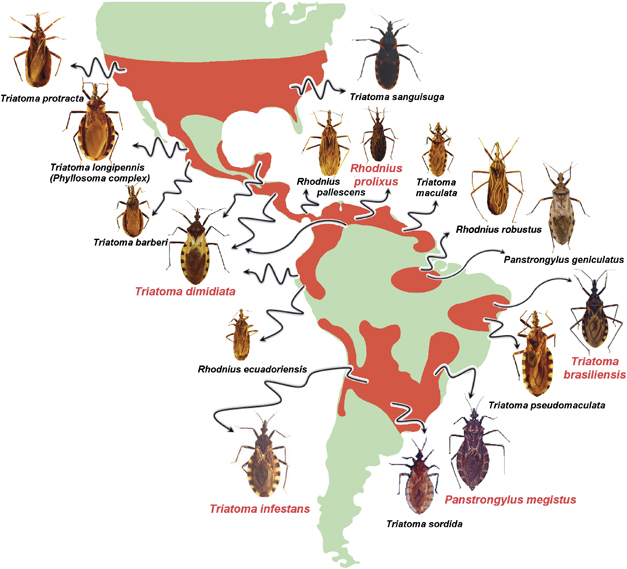
\includegraphics[height=.9\textheight]{slides/triatomine-map.jpg}
\end{frame}

%%%%%%%%%%%%%%%%%%%%%%%%%%%%%%%%%%%%%%%%%%%%%%%%%%%%%%%%%%%%%%%%%%%%%%%%%%%%%%%%%%%%%%%%%%%%%%%%%%%%%%%%%%%%
\begin{frame}{Chagas en Argentina}
	\begin{columns}
		\begin{column}{0.45\textwidth}
			% In Argentina, the disease is endemic in the \textit{Gran Chaco} region and
			% also predominant in communities with migrations from this area.
			La enfermedad es endémica de la zona del Gran Chaco
			% y tambi\'en predominante en algunas comunidades que han migrado de esta zona.

			\medskip Las estimaciones de usuarios infectados oscilan alrededor de 1.5 millones de personas con solo 1 a 2 mil tratamientos realizados por año. En 2009 los tests de seroprevalencia en embarazadas alcanzaba el 4.2\% de casos.

			\medskip
			 % infected users and only 1 to 2 thousand treatments done yearly, where 30\% of all infected will develop a cardiopathy.
			% % % %DECIR ORAL: Seroprevalence tests in pregnant women reached 4.2% in 2009 which predicted 1.300 infected newborns that year.

		\end{column}
		\begin{column}{0.45\textwidth}
			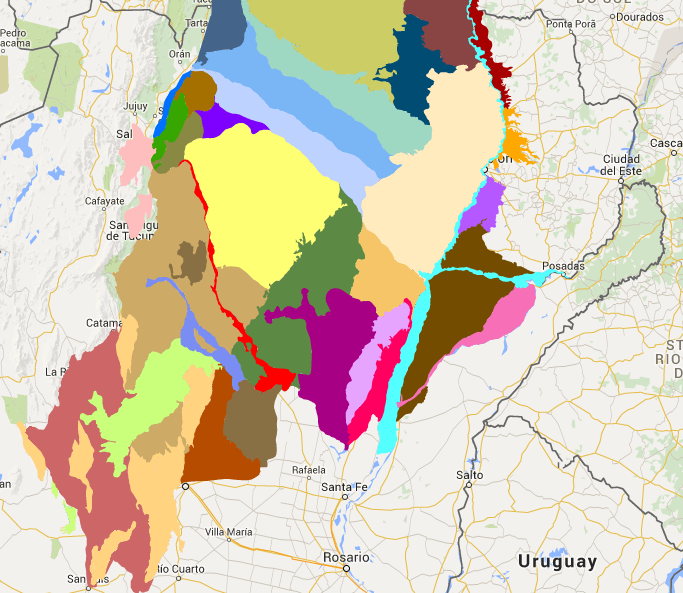
\includegraphics[height=.7\textheight]{slides/Ambientes_GranChaco_TNC-Argentina.png}
		\end{column}
	\end{columns}
\end{frame}

%%%%%%%%%%%%%%%%%%%%%%%%%%%%%%%%%%%%%%%%%%%%%%%%%%%%%%%%%%%%%%%%%%%%%%%%%%%%%%%%%%%%%%%%%%%%%%%%%%%%%%%%%%%%
\begin{frame}{Chagas en México}
	\begin{columns}
		\begin{column}{0.3\textwidth}

			La enfermedad es endémica en algunas regiones y estados particulares
			 % is endemic in some particular states of the country, shown in the map.
			%The disease is endemic in the states of Jalisco, Oaxaca, Veracruz, Guerrero, Morelos, Puebla, Hidalgo and Tabasco.
			%This selection was based on the top 25\% prevalance states.

			% \medskip Non official reports estimate 5.5 million of potentially affected people and studies indicate that less than 0.5\% of infected have access to treatments.

			\medskip No oficialmente, los reportes estiman 5.5 millones de personas potencialmente afectados y donde menos del 0.5\% de los infectados tienen acceso a tratamientos
			 % official reports estimate 5.5 million of potentially affected people and studies indicate that less than 0.5\% of infected have access to treatments.


		\end{column}
		\begin{column}{0.7\textwidth}
			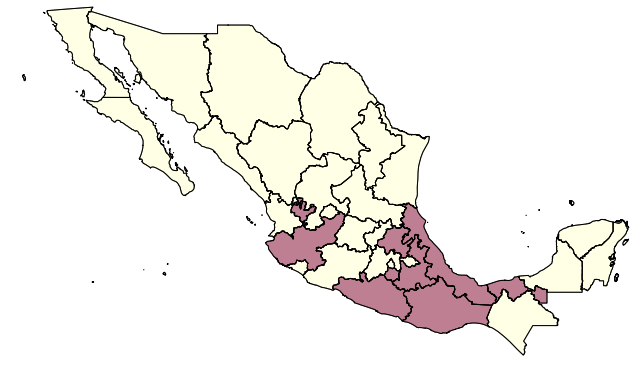
\includegraphics[width=\textwidth]{slides/Ambientes_Gran_Chaco-Mexico_original.png}
		\end{column}
	\end{columns}
\end{frame}
%%%%%%%%%%%%%%%%%%%%%%%%%%%%%%%%%%%%%%%%%%%%%%%%%%%%%%%%%%%%%%%%%%%%%%%%%%%%%%%%%%%%%%%%%%%%%%%%%%%%%%%%%%%%

\begin{frame}{Puntos claves}
	% Chagas is a disease:
	El Chagas es una enfermedad:
	\begin{itemize}
		\item \ldots con diferentes vías de transmisión y donde las \textbf{migraciones de largo plazo} juegan un papel clave
		%explicar vertical, congenita y transfusion/transplante
		\item \ldots donde un pequeño número de la población infectada sabe que la está padeciendo
		% for which a low proportion of the infected population knows that they have the disease.
		\item \ldots con una fase asintomática que puede extenderse más de 10 años
		% % ORALLY SAY: 30 years of vector mitigation activities in GC.
		\item \ldots que es epidémica y desatendida
		% \item ... which is epidemic and unattended.
	\end{itemize}
	En particular, la fundación busca encontrar chagásicos en zonas no tradicionalmente endémicas
	%Es decir, gente de fuera de Gran Chaco infectada con \textit{Trypanosoma Cruzi} (el parásito que causa el Chagas).
\end{frame}


%%%%%%%%%%%%%%%%%%%%%%%%%%%%%%%%%%%%%%%%%%%%%%%%%%%%%%%%%%%%%%%%%%%%%%%%%%%%%%%%%%%%%%%%%%%%%%%%%%%%%%%%%%%%%
\begin{frame}{Objetivo}
	\begin{block}{\ldots atacar problemáticas de América Latina relacionadas con el Chagas}

	% The purpose of this work is to support ongoing national health campaigns
	% by analyzing mobility information contained in Call Detail Records.
	Este trabajo propone un modelo que utiliza información de registros (logs) de llamados telefónicos
	como forma de observar en qué regiones del país se espera encontrar una alta proporción de personas chagásicas

	\bigskip
	Sabiendo que las migraciones humanas tienen un rol crucial en la diseminación de la enfermedad, el modelo busca
	detectar migraciones a partir de los patrones de uso celular
	% , donde, idealmente, se vea que una fluida comunicación con el lugar de orígen es indicador

	\bigskip
	Idealmente podremos encontrar aquellos indicadores de usuarios que mejor determinen las zonas del país tradicionalmente no-endémicas, donde exista más intercambio migratorio con la zona del Gran Chaco
	% We strongly assume that long-term migrations are related to fluid communications with the past area of residence.
	\end{block}
\end{frame}


%% HABLAR de pre trabajos en vih y malaria en el D4D? .
%


%%%%%%%%%%%%%%%%%%%%%%%%%%%%%%%%%%%%%%%%%%%%%%%%%%%%%%%%%%%%%%%%%%%%%%%%%%%%%%%%%%%%%%%%%%%%%%%%%%%%%%%%%%%%
\section{Fuentes de Datos}
%%%%%%%%%%%%%%%%%%%%%%%%%%%%%%%%%%%%%%%%%%%%%%%%%%%%%%%%%%%%%%%%%%%%%%%%%%%%%%%%%%%%%%%%%%%%%%%%%%%%%%%%%%%%


\begin{frame}{Visualización Social: El grafo de comuniaciones}

	\center\
	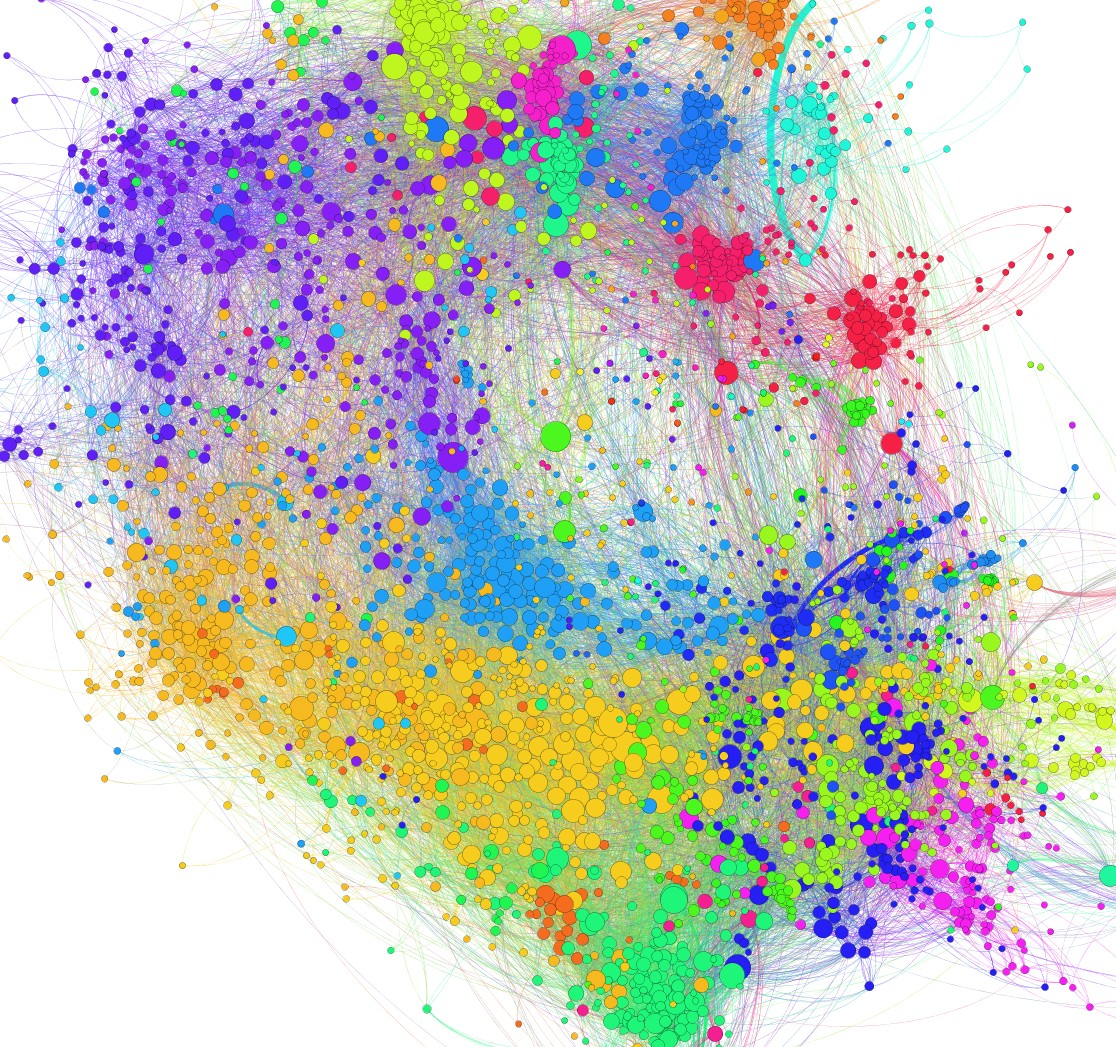
\includegraphics[width = 1.0 \textwidth, trim = 0 0 0 0cm, clip = true]
	{slides/Graph-screenshot.jpg}

\end{frame}

%%%%%%%%%%%%%%%%%%%%%%%%%%%%%%%%%%%%%%%%%%%%%%%%%%%%%%%%%%%%%%%%%%%%%%%%%%%%%%%%%%%%%%%%%%%%%%%%%%%%%%%%%%%%
\begin{frame}{Datos de Telefonia Celular (CDRs)}

% \begin{block}{Los datos: CDRs}

Los conjuntos de datos consisten de registros detallados de llamados (CDRs) para Mexico y Argentina con una TelCo distinta por pais. El primero tiene 24 meses de datos mientras que el segundo 5 meses.

%Nuestro conjunto de datos consiste en 5 meses de registros de llamados (CDRs) \textbf{anonimizados} de una compañía telefónica en la \textbf{Rep\'ublica Argentina}.

\medskip
Podemos representar cada registro en una tupla $\left < i, j, t, d, l \right >$ que contiene :
\begin{itemize}
	\item Usuarioss $i$ y $j$ en esa llamada
	%Usuarios anonimizados de origen y destino de la llamada.
	\item Tiempo de inicio y duración de la llamada $t$
	\item Direccion $d$ de la llamada (entrante o saliente, con respecto a $i$)
	\item $l$ es el ID de la antena telefónica usada por $i$ en esa comunicación
\end{itemize}

\medskip

Cada dataset tiene mas de 9 mil millones de registros de llamadas geolocalizadas. La 

In all, each dataset has more than 9 billion geolocalized calls in each dataset. The population coverage of each telco is of 8 million and 2 million mobile lines for the argentinean and mexican datasets respectively.
%En total son m\'as de 9,000,000,000 llamados geolocalizados de 40,000,000 millones de l\'ineas celulares. % a las cuales analizaremos sus patrones de comunicaciones.

\medskip
The antenna datasets consists of more than five thousand geolocalized antennas.
%Contamos además con la lista de antenas celulares, con su correspondiente geolocalización (latitud y longitud).

% \end{block}
\end{frame}

%%%%%%%%%%%%%%%%%%%%%%%%%%%%%%%%%%%%%%%%%%%%%%%%%%%%%%%%%%%%%%%%%%%%%%%%%%%%%%%%%%%%%%%%%%%%%%%%%%%%%%%%%%%%
\section{ Descripción de los datos}
%%%%%%%%%%%%%%%%%%%%%%%%%%%%%%%%%%%%%%%%%%%%%%%%%%%%%%%%%%%%%%%%%%%%%%%%%%%%%%%%%%%%%%%%%%%%%%%%%%%%%%%%%%%%



%%%%%%%%%%%%%%%%%%%%%%%%%%%%%%%%%%%%%%%%%%%%%%%%%%%%%%%%%%%%%%%%%%%%%%%%%%%%%%%%%%%%%%%%%%%%%%%%%%%%%%%%%%%%
%%%%%%%%%%%%%%%%%%%%%%%%%%%%%%%%%%%%%%%%%%%%%%%%%%%%%%%%%%%%%%%%%%%%%%%%%%%%%%%%%%%%%%%%%%%%%%%%%%%%%%%%%%%%

% Procedimiento:
	% Obtener la lista de antenas de GC
	% Determinar la casa de los usuarios
	% Determinar, para cada usuario, si se comunicó con un habitante de GC
	% Determinar las agregaciones por antena
	% Visualizar(agrego alfa, min_volume y zoom en regiones)

\begin{frame}{Methodology (1)}

	\begin{block}{Home Prediction}
		\begin{itemize}
			\item As a first step, we determined each user's residence antenna. This was chosen to be the most used frequently used antenna during week evenings.
			%Como primer paso, determinamos para cada usuario, su lugar de residencia.

			%La antena elegida como hogar es la más frecuentemente usada,
			%considerando llamados nocturnos en días de semana.

			%\item The hypothesis:
			%La hipótesis: la mayoría de los días, las personas se encuentran en sus casas durante la noche.

			%\bigskip
			%Así, cada antena queda asociada a un conjunto de usuarios: sus \textit{habitantes}.
			\item Users for which the inferred home antenna is located in an \textit{endemic area} will
			be considered the set of \textit{endemic users}.
			%Nota: Los usuarios cuya antena inferida pertenece al Gran Chaco (la zona de riesgo)
			%se consideran el conjunto de \textit{habitantes de Gran Chaco}.

		\end{itemize}
	\end{block}
	\pause\
	\begin{block}{Aggregation of vulnerable users}
		\begin{itemize}
			%\item For every user, we listed all of his call receivers in a given month.
			%Para cada usuario, obtuvimos la lista de todos los usuarios con los que se comunicó. %ojo que esto podria cambiar en versiones posteriores cuando cambie la definicion de 'vulnerable'

			\item If a given user communicated with the \textit{endemic area} in the selected period of time, we tagged him as potentially \textit{vulnerable}.

			%Si un usuario tuvo comunicaciones con la zona endémica (Gran Chaco), se considera que tiene mayor riesgo de tener Mal de Chagas, y lo marcamos como potentialmente \textit{vulnerable}.

			\item  We aggregated vulnerable users and total users (residents) per antenna.
			%Agregamos usuarios vulnerables y usuarios totales (habitantes) para cada antena.

			%\item We also aggregated the total volume of outgoing calls from every antenna and from these we extracted every call that had a user whose home is in the \textit{endemic area} as a receiver (\textit{vulnerable calls}).
			%Tambien agregamos el volumen total de llamados salientes de cada antena,
			%y de estos, los que tenían un habitante de Gran Chaco como destinatario (\textit{llamados vulnerables}).

			%\bigskip
			%Por lo tanto se obtuvieron, para cada antena, cuatro indicadores:
			%\begin{itemize}
			%	\item Cantidad de usuarios habitantes
			%	\item Cantidad de usuarios vulnerables entre los habitantes.
			%	\item Volumen de llamados salientes
			%	\item Volumen de llamados vulnerables salientes.
			%\end{itemize}
		\end{itemize}
	\end{block}
\end{frame}

%%%%%%%%%%%%%%%%%%%%%%%%%%%%%%%%%%%%%%%%%%%%%%%%%%%%%%%%%%%%%%%%%%%%%%%%%%%%%%%%%%%%%%%%%%%%%%%%%%%%%%%%%%%%
\begin{frame}{Methodology (2)}


	\begin{block}{Mapas de calor}


		We generated heat maps from these results, plotting a colored circle around each antenna, which encodes its \textit{vulnerable} communication patterns.
		%A partir de los datos obtenidos, generamos mapas de calor que representan las comunicaciones de la celda con el Gran Chaco.

		% DECIR: en este trabajo encnotramos areas de alta interaccion con lazona endemica a traves de analizar los mapas de calor entre ls residentes de una zona con otra.

		%Generamos un c\'irculo por cada celda donde:
		\begin{itemize}
			\item the \textbf{area} depends on the on the volume of use.
			%el \textbf{\'area} depende de la cantidad de usuarios (habitantes),
			\item the \textbf{color} corresponds to the percentage of vulnerable use in that antenna (whether calls or users).
			%el \textbf{color} corresponde al porcentaje de usuarios vulnerables que viven en esa antena.
		\end{itemize}

	\end{block}

	\begin{block}{Antenna Filter}
		$\beta$ will be our parameter to filter antennas by minimum vulnerable interaction rates.
%		We added two filtering thresholds $\beta$ and $min\_volumen$ which will control the antennas to be plotted if the percentage and volume of vulnerable interactions for that cell are higher than their respective thresholds.
		%Every antenna will be plotted if:
		% Notar que en ningún lado antes de esto dijimos que íbamos a pintar un mapa de Argentina con las antenas.
		%Dos par\'ametros $\beta$ y $min\_volumen$  filtran la lista de antenas a ser visualizadas.
		%Cada antena se grafica si:
		%\begin{itemize}
		%	\item the percentage of vulnerable users/calls is bigger than  $\beta$.
			%el porcentaje de usuarios vulnerables es mayor que $\beta$,
		%	\item the volume of vulnerable users/calls is bigger than $min\_volumen$.
			%el volumen de uso vulnerable es mayor que $min\_volumen$ de llamados o usuarios.
		%\end{itemize}

		%
		%\bigskip
		%Por lo tanto, el modelo permitiría ver las antenas donde existen mayores lazos familiares con el Gran Chaco.	% Creo que 'familiares' es muy fuerte

		%\bigskip
		%A\'un con los par\'ametros anteriores, fue necesario separar el filtrado por distintas regiones:
		%
		%\smallskip
		%Una antena de baja proporción a nivel nacional ($\beta=10\%$) puede ser llamativa, por ejemplo, en Tierra del Fuego.
		%%aca se inserta imagen x ejemplo?? %No, la imagen es demasiado grande me parece. Lo podemos discutir.

	\end{block}
\end{frame}

%%%%%%%%%%%%%%%%%%%%%%%%%%%%%%%%%%%%%%%%%%%%%%%%%%%%%%%%%%%%%%%%%%%%%%%%%%%%%%%%%%%%%%%%%%%%%%%%%%%%%%%%%%%%
\section{Exploración de los datos}
%%%%%%%%%%%%%%%%%%%%%%%%%%%%%%%%%%%%%%%%%%%%%%%%%%%%%%%%%%%%%%%%%%%%%%%%%%%%%%%%%%%%%%%%%%%%%%%%%%%%%%%%%%%%



%%%%%%%%%%%%%%%%%%%%%%%%%%%%%%%%%%%%%%%%%%%%%%%%%%%%%%%%%%%%%%%%%%%%%%%%%%%%%%%%%%%%%%%%%%%%%%%%%%%%%%%%%%%%
\begin{frame}
	\frametitle{Mapa de calor: Argentina, $\beta$ = 1 \%}
	\center\
	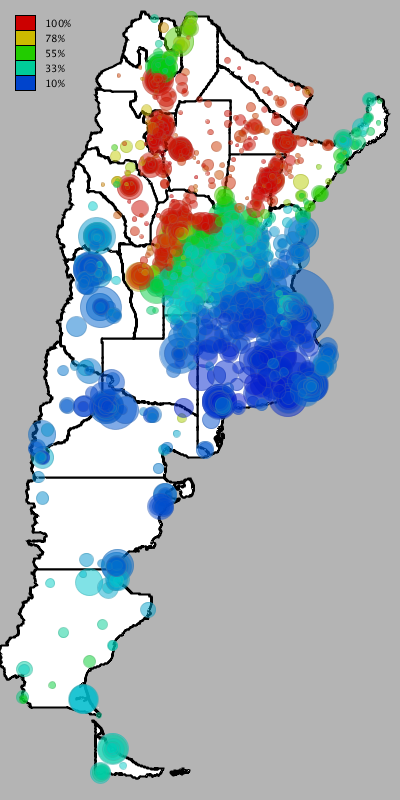
\includegraphics[height=.9\textheight,width = .9\columnwidth, keepaspectratio]
	{slides/201112_hi_res_argentina_usuarios_proporcion_circulos_beta1.png}
\end{frame}

%%%%%%%%%%%%%%%%%%%%%%%%%%%%%%%%%%%%%%%%%%%%%%%%%%%%%%%%%%%%%%%%%%%%%%%%%%%%%%%%%%%%%%%%%%%%%%%%%%%%%%%%%%%%
\begin{frame}
	\frametitle{Mapa de calor: Argentina, $\beta$ = 15 \%}
	\center\
	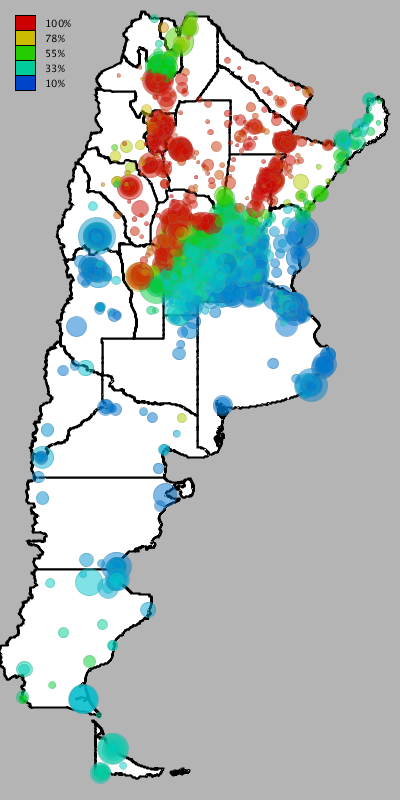
\includegraphics[height=.9\textheight,width = .9\columnwidth, keepaspectratio]
	{slides/201112_hi_res_argentina_usuarios_proporcion_circulos_beta15.png}
\end{frame}

%%%%%%%%%%%%%%%%%%%%%%%%%%%%%%%%%%%%%%%%%%%%%%%%%%%%%%%%%%%%%%%%%%%%%%%%%%%%%%%%%%%%%%%%%%%%%%%%%%%%%%%%%%%%
\begin{frame}
	\frametitle{Mapa de calor: Argentina, $\beta$ = 30 \%}
	\center\
	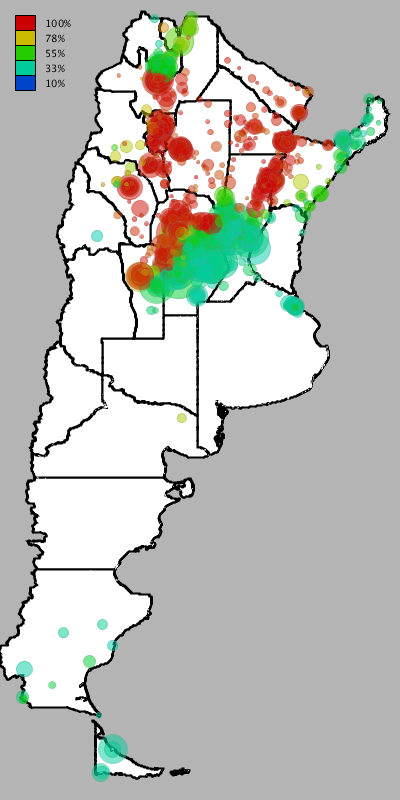
\includegraphics[height=.9\textheight,width = .9\columnwidth, keepaspectratio]
	{slides/201112_hi_res_argentina_usuarios_proporcion_circulos_beta30.png}
\end{frame}

%%%%%%%%%%%%%%%%%%%%%%%%%%%%%%%%%%%%%%%%%%%%%%%%%%%%%%%%%%%%%%%%%%%%%%%%%%%%%%%%%%%%%%%%%%%%%%%%%%%%%%%%%%%%
\begin{frame}
	\frametitle{Mapa de calor: Argentina, $\beta$ = 50 \%}
	\center\
	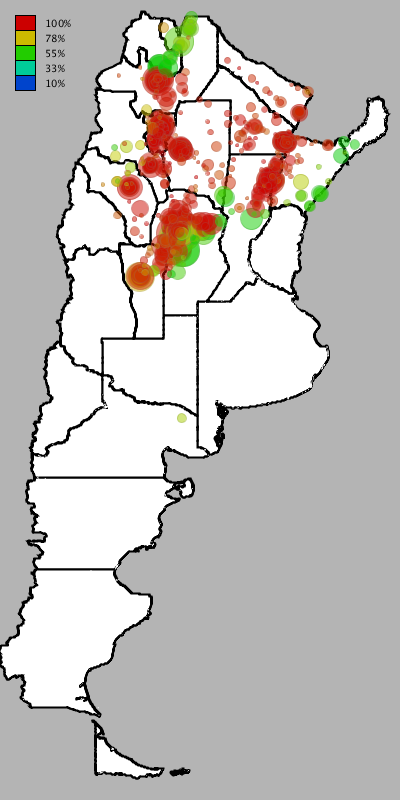
\includegraphics[height=.9\textheight,width = .9\columnwidth, keepaspectratio]
	{slides/201112_hi_res_argentina_usuarios_proporcion_circulos_beta50.png}
\end{frame}

%%%%%%%%%%%%%%%%%%%%%%%%%%%%%%%%%%%%%%%%%%%%%%%%%%%%%%%%%%%%%%%%%%%%%%%%%%%%%%%%%%%%%%%%%%%%%%%%%%%%%%%%%%%%

\setbeamercolor{background canvas}{bg=white}

\begin{frame}{Regiones focalizadas}
	A partir de estas primeras visualizaciones, con la gente de la fundación decidimos focalizar la granularidad en regiones específicas y fuera del Gran Chaco.
	%A partir de estos primeros mapas se decidi\'o enfocar la visualizaci\'on y mejorar la precisi\'on en ciertas regiones fuera del Gran Chaco.
		\begin{itemize}
			\item Tierra del Fuego
			\item Este de Río Negro
			\item Buenos Aires
			\item Capital Federal, South and North CABA, and AMBA
			\item Córdoba Central
		\end{itemize}
\end{frame}

%%%%%%%%%%%%%%%%%%%%%%%%%%%%%%%%%%%%%%%%%%%%%%%%%%%%%%%%%%%%%%%%%%%%%%%%%%%%%%%%%%%%%%%%%%%%%%%%%%%%%%%%%%%%
\begin{frame}
	\frametitle{Mapa de calor: AMBA, $\beta$ = 2 \%}
	\centering
	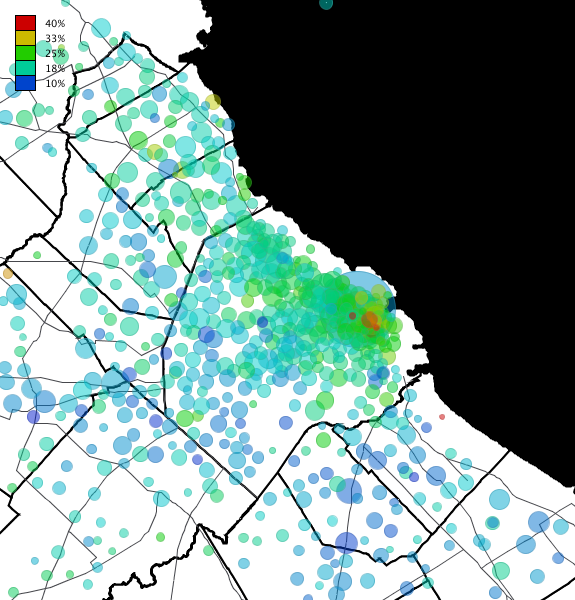
\includegraphics[height=.9\textheight,width = .9\columnwidth,keepaspectratio]
	{slides/201112_hi_res_amba_usuarios_proporcion_circulos_beta2.png}
\end{frame}
%%%%%%%%%%%%%%%%%%%%%%%%%%%%%%%%%%%%%%%%%%%%%%%%%%%%%%%%%%%%%%%%%%%%%%%%%%%%%%%%%%%%%%%%%%%%%%%%%%%%%%%%%%%%
\begin{frame}
	\frametitle{Mapa de calor: AMBA, $\beta$ = 10 \%}
	\centering
	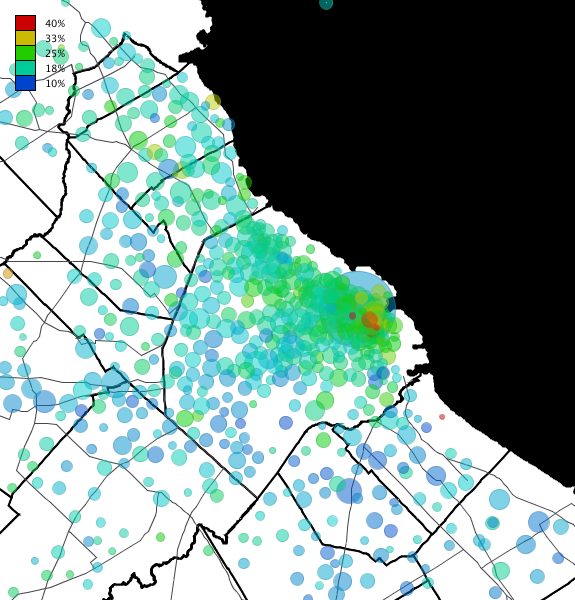
\includegraphics[height=.9\textheight,width = .9\columnwidth,keepaspectratio]
	{slides/201112_hi_res_amba_usuarios_proporcion_circulos_beta10.png}
\end{frame}
%%%%%%%%%%%%%%%%%%%%%%%%%%%%%%%%%%%%%%%%%%%%%%%%%%%%%%%%%%%%%%%%%%%%%%%%%%%%%%%%%%%%%%%%%%%%%%%%%%%%%%%%%%%%
\begin{frame}
	\frametitle{Mapa de calor: AMBA, $\beta$ = 20 \%}
	\centering
	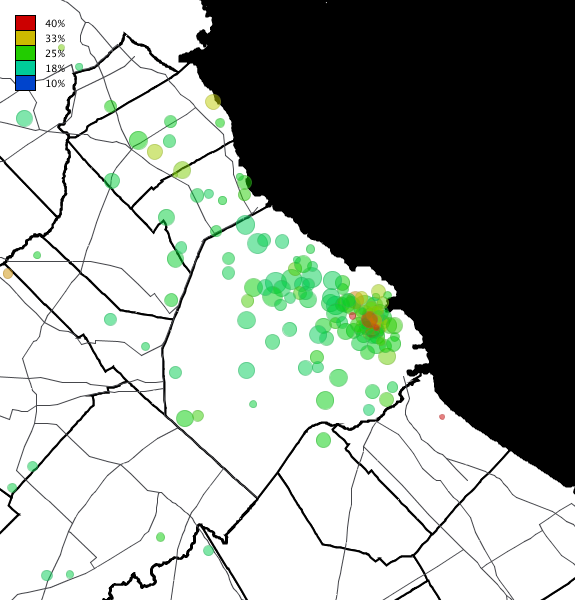
\includegraphics[height=.9\textheight,width = .9\columnwidth,keepaspectratio]
	{slides/201112_hi_res_amba_usuarios_proporcion_circulos_beta20.png}
\end{frame}
%%%%%%%%%%%%%%%%%%%%%%%%%%%%%%%%%%%%%%%%%%%%%%%%%%%%%%%%%%%%%%%%%%%%%%%%%%%%%%%%%%%%%%%%%%%%%%%%%%%%%%%%%%%%
\begin{frame}
	\frametitle{Heat Map AMBA, $\beta$ = 28 \%}
	\centering
	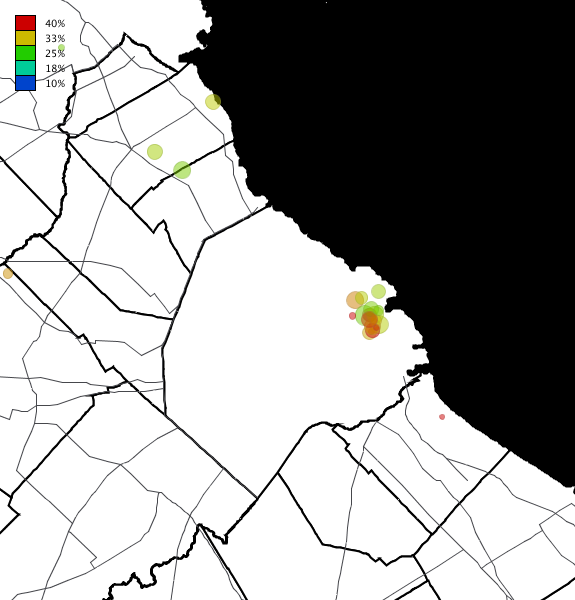
\includegraphics[height=.9\textheight,width = .9\columnwidth,keepaspectratio]
	{slides/201112_hi_res_amba_usuarios_proporcion_circulos_beta28.png}
\end{frame}
%%%%%%%%%%%%%%%%%%%%%%%%%%%%%%%%%%%%%%%%%%%%%%%%%%%%%%%%%%%%%%%%%%%%%%%%%%%%%%%%%%%%%%%%%%%%%%%%%%%%%%%%%%%%

\begin{frame}{Comunidades resaltadas}
	Luego de filtrar los mapas y explorar con distintas visualizaciones, encontramos antentas especificas que se resaltan por su nivel de vulnerabilidad
	%Como resultado del filtrado en cada zona, nos hemos quedado con las antenas destacadas por su nivel de riesgo y, utilizando su ubicaci\'on, las emparejamos con localidades o comunidades argentinas.

	\bigskip

	\begin{block}{Ejemplos de comunidades en Argentina}
		\begin{itemize}
			\item Cordoba: Freyre, La Tordilla, Balnearia
			%hay muchas mas pero no se si esta bien poner esto
			\item AMBA: Avellaneda, Parque Patricios, San Isidro
			\item Provincia de Buenos Aires: Lima, San Nicolas
			\item La Rioja: Chamical y Malanz\'an
			\item Salta: Tartagal
		\end{itemize}

	\end{block}
\end{frame}


%%%%%%%%%%%%%%%%%%%%%%%%%%%%%%%%%%%%%%%%%%%%%%%%%%%%%%%%%%%%%%%%%%%%%%%%%%%%%%%%%%%%%%%%%%%%%%%%%%%%%%%%%%%%
\section{Clasificacion Supervisada}
%%%%%%%%%%%%%%%%%%%%%%%%%%%%%%%%%%%%%%%%%%%%%%%%%%%%%%%%%%%%%%%%%%%%%%%%%%%%%%%%%%%%%%%%%%%%%%%%%%%%%%%%%%%%

\begin{frame}{Notacion}
%	\begin{columns}
%		\begin{column}{0.20 \textwidth}
			\begin{block}{Target Variable}
			Let $T_0$ and $T_1$ be time periods corresponding to $($01/01/14, 31/07/15 $)$ and $($01/08/15, 31/12/15$)$ respectively.

			Consider $U_0$ to be the set of users that lived in the \textbf{mexican} endemic region $E_Z$ during period $T_0$. Then our target variable $Y$ for every user $u$ is:
			\[
			%\begin{equation}
			Y_u =
			\begin{cases}
			&1 \ \mbox{if} \ u \in U_0  \\
			&0 \ \mbox{in other cases}.
			\end{cases}
			%\end{equation}
			\]
			where $\ u \in U_0$ iff the user's home antenna is in $E_Z$ during $T_0$.
			\end{block}

\end{frame}
%%%%%%%%%%%%%%%%%%%%%%%%%%%%%%%%%%%%%%%%%%%%%%%%%%%%%%%%%%%%%%%%%%%%%%%%%%%%%%%%%%%%%%%%%%%%%%%%%%%%%%%%%%%%

\begin{frame}{Definiciones}
%	\begin{columns}
%		\begin{column}{0.20 \textwidth}
			\begin{block}{Foo}
			Bar 
			\[
			%\begin{equation}
			Y_u =
			\begin{cases}
			&1 \ \mbox{si} \ u \in U_0  \\
			&0 \ \mbox{en otros casos}.
			\end{cases}
			%\end{equation}
			\]
			where $\ u \in U_0$ iff the user's home antenna is in $E_Z$ during $T_0$.
			\end{block}

\end{frame}
%%%%%%%%%%%%%%%%%%%%%%%%%%%%%%%%%%%%%%%%%%%%%%%%%%%%%%%%%%%%%%%%%%%%%%%%%%%%%%%%%%%%%%%%%%%%%%%%%%%%%%%%%%%%

\begin{frame}{Mobility Classifier}
%	\begin{columns}
%		\begin{column}{0.20 \textwidth}
			\begin{block}{Target Variable}
			Let $T_0$ and $T_1$ be time periods corresponding to $($01/01/14, 31/07/15 $)$ and $($01/08/15, 31/12/15$)$ respectively.

			Consider $U_0$ to be the set of users that lived in the \textbf{mexican} endemic region $E_Z$ during period $T_0$. Then our target variable $Y$ for every user $u$ is:
			\[
			%\begin{equation}
			Y_u =
			\begin{cases}
			&1 \ \mbox{if} \ u \in U_0  \\
			&0 \ \mbox{in other cases}.
			\end{cases}
			%\end{equation}
			\]
			where $\ u \in U_0$ iff the user's home antenna is in $E_Z$ during $T_0$.
			\end{block}

\end{frame}

%%%%%%%%%%%%%%%%%%%%%%%%%%%%%%%%%%%%%%%%%%%%%%%%%%%%%%%%%%%%%%%%%%%%%%%%%%%%%%%%%%%%%%%%%%%%%%%%%%%%%%%%%%%%
\begin{frame}{Feature Matrix Description}
	The features were constructed using data during the period $T_0$ and amount to a total of 130 variables per user.

	\begin{itemize}
		\item Volume of ten most used antennas.
		\item Mobility diameter.
		%Presentamos una utilizaci\'on novedosa de los CDRs (Call Detail Records), datos que
		%fueron recogidos para otro fin (facturación).
		\item Graph data and communications, segmented accordingly:
		\begin{itemize}
			\item Month of interaction.
			\item Time of the week.
			\item Vulnerability of the interactions.
			\item Duration, volume and direction of the interactions.
		\end{itemize}
	\end{itemize}

	\begin{block}{Correlaciones entre atributos y targets}

	As expected, there was a high Pearson correlation between $Y$ and calling patterns with the endemic region.
	%All of them being above \($0.7$\).
	\end{block}

\end{frame}

%%%%%%%%%%%%%%%%%%%%%%%%%%%%%%%%%%%%%%%%%%%%%%%%%%%%%%%%%%%%%%%%%%%%%%%%%%%%%%%%%%%%%%%%%%%%%%%%%%%%%%%%%%%%

\begin{frame}{ ML setup}
			Standard industry classifiers were fit with
			and 5-Fold cross validation and a 10\% hold out set for scoring.

			\medskip

			All standard metrics used rated higher than $0.96$. The lowest of them being the weighted F1 score with $0.964$.

%		\end{block}
%		\begin{block}{Scores}
%		\end{block}
%
\end{frame}


%%%%%%%%%%%%%%%%%%%%%%%%%%%%%%%%%%%%%%%%%%%%%%%%%%%%%%%%%%%%%%%%%%%%%%%%%%%%%%%%%%%%%%%%%%%%%%%%%%%%%%%%%%%%
\section{Resultados}
%%%%%%%%%%%%%%%%%%%%%%%%%%%%%%%%%%%%%%%%%%%%%%%%%%%%%%%%%%%%%%%%%%%%%%%%%%%%%%%%%%%%%%%%%%%%%%%%%%%%%%%%%%%%

%%%%%%%%%%%%%%%%%%%%%%%%%%%%%%%%%%%%%%%%%%%%%%%%%%%%%%%%%%%%%%%%%%%%%%%%%%%%%%%%%%%%%%%%%%%%%%%%%%%%%%%%%%%%
% Resultados:
%
%
%
%

\begin{frame}{Foo}
	\begin{block}{Bar}
		Baz
		\medskip
		foo
	\end{block}

	\pause\

	\begin{block}{foo}
		varrr

		\medskip
			asdf

		\medskip
		alala

		\medskip
		foo
	\end{block}
\end{frame}


%%%%%%%%%%%%%%%%%%%%%%%%%%%%%%%%%%%%%%%%%%%%%%%%%%%%%%%%%%%%%%%%%%%%%%%%%%%%%%%%%%%%%%%%%%%%%%%%%%%%%%%%%%%%
\section{Conclusiones}
%%%%%%%%%%%%%%%%%%%%%%%%%%%%%%%%%%%%%%%%%%%%%%%%%%%%%%%%%%%%%%%%%%%%%%%%%%%%%%%%%%%%%%%%%%%%%%%%%%%%%%%%%%%%

%%%%%%%%%%%%%%%%%%%%%%%%%%%%%%%%%%%%%%%%%%%%%%%%%%%%%%%%%%%%%%%%%%%%%%%%%%%%%%%%%%%%%%%%%%%%%%%%%%%%%%%%%%%%
% Conclusiones:


\begin{frame}{Conclusiones Esperadas}

	Los mapas de calor muestran un descenso de temperatura desde el ``Gran Chaco'' hacia afuera
	% , indicando que las antenas descienden su porcentaje de usuarios \textit{vulnerables}

	\medskip
	Los atributos de llamados desde y hacia la región endémica son relevantes para predecir migraciones
	% , lo cual confirma nuestra hipótesis utilizada para construir los mapas de calor

	\medskip
	Fue posible construir clasificadores de alta performance para detectar cuáles usuarios migraron desde la región endémica
	% , sobre todos los usuarios actualmente no endémico

\end{frame}

%%%%%%%%%%%%%%%%%%%%%%%%%%%%%%%%%%%%%%%%%%%%%%%%%%%%%%%%%%%%%%%%%%%%%%%%%%%%%%%%%%%%%%%%%%%%%%%%%%%%%%%%%%%%
%%%%%%%%%%%%%%%%%


\begin{frame}{Conclusiones Inesperadas}

	Los mapas ayudaron a detectar comunidades con alta interaccion vulnerable fuera de la zona endemica

	\medskip
	Los mejores clasificadores fueron los de ensamble
	% en estrategias que no son intrusivas a las personas

	\medskip
	Salvo el clasificador de ``Naive Bayes'', la performance fue muy baja para la metrica $F1$ en el problema 2

	\medskip
	Los tres tipos de atributos más relevantes para la clasificaición de los migrantes estaban relacionadas con:

	\begin{enumerate*}[label={\alph*)},]
		\item la mobilidad del usuario
		\item las interacciones y patrones de llamados con vecinos vulnerables, y
		\item uso celular en los meses más cercanos a $T_0$, así como también la actividad en el mes de Diciembre.
	\end{enumerate*}

\end{frame}

%%%%%%%%%%%%%%%%%%%%%%%%%%%%%%%%%%%%%%%%%%%%%%%%%%%%%%%%%%%%%%%%%%%%%%%%%%%%%%%%%%%%%%%%%%%%%%%%%%%%%%%%%%%%
%%%%%%%%%%%%%%%%%

\begin{frame}{Reciclaje de CDRs}
	    
	    Presentamos una utilizaci\'on novedosa de los CDRs, datos que inicialmente se utilizan para fines de facturación
		\medskip
		Se puede extender hacia otras regiones y otras epidemias de características similares
		\medskip
		
\end{frame}

%%%%%%%%%%%%%%%%%%%%%%%%%%%%%%%%%%%%%%%%%%%%%%%%%%%%%%%%%%%%%%%%%%%%%%%%%%%%%%%%%%%%%%%%%%%%%%%%%%%%%%%%%%%%
%%%%%%%%%%%%%%%%%

\begin{frame}{Inconvenientes}

		\begin{block}{Sesgos en los datos}
			\begin{itemize}
			\item Basados únicamente en datos de una sola TelCo por país que no capturan migraciones internacionales 
			%La caracterizaci\'on actual de la vulnerabilidad viene dada por contacto telefónicos con usuarios de antenas del Gran Chaco.
			\item Concentración geoespacial de usuarios
			
			\item Mobilidad no implica prevalencia
			
			\item Estacionalidades en las migraciones

			\end{itemize}
 	 	\end{block}
\end{frame}


  %%%%%%%%%%%%%%%%%%%%%%%%%%%%%%%%%%%%%%%%%%%%%%%%%%%%%%%%%%%%%%%%%%%%%%%%%%%%%%%%%%%%%%%%%%%%%%%%%%%%%%%%%%%%

 \begin{frame}{Lineas Futuras de Trabajo}


	\begin{block}{Extensiones}
		Probar otros clasificadores y metodos para hallar los atributos mas relevantes en terminos de migraciones. Tambien se podria mejorar el analisis pudiendo mejorar el preprocesamiento de los datos con cuestioens de estacionaridad o de tecnicas de ``Feature Engineering''.
	\end{block}

	\medskip

	\begin{block}{Nuevas fuentes de datos}
		Agreagar informacion para mayores analisis:
		\begin{itemize}
			\item Comparacion de resultados de movilidad con serologia por region
			\item Categorizacion de antenas por grado de ruralidad del ambiente
			\item infected newborns
			\item acute Chagas cases.
			\item serological data per community, amongst others.
		\end{itemize}
	\end{block}


 \end{frame}
%


%%%%%%%%%%%%%%%%%%%%%%%%%%%%%%%%%%%%%%%%%%%%%%%%%%%%%%%%%%%%%%%%%%%%%%%%%%%%%%%%%%%%%%%%%%%%%%%%%%%%%%%%%%%%
% ==============================================

\begin{frame}{Gracias! }
	\begin{columns}
		\begin{column}{0.20 \textwidth}
		\end{column}
		\begin{column}{0.55 \textwidth}
				\center\
				Juan Mateo de Monasterio \\
				\textit{laterio@gmail.com} \\
		\end{column}
	\end{columns}
\end{frame}

% ==============================================

\justifying%
\scalefont{0.7}
\bibliographystyle{unsrtnat}
\bibliography{./}

% \end{columns}
% ==============================================

\vfill

\end{document}




%   ___  _     ___         ___________ __ __ _____ _____
%  /   \| |   |   \       / ___/      |  |  |     |     |
% |     | |   |    \     (   \_|      |  |  |   __|   __|
% |  O  | |___|  D  |     \__  |_|  |_|  |  |  |_ |  |_
% |     |     |     |     /  \ | |  | |  :  |   _]|   _]
% |     |     |     |     \    | |  | |     |  |  |  |
%  \___/|_____|_____|      \___| |__|  \__,_|__|  |__|

%%%%%%%%%%%%%%%%%%%%%%%%%%%%%%%%%%%%%%%%%%%%%%%%%%%%%%%%%%%%%%%%%%%%%%%%%%%%%%%%%%%%%%%%%%%%%%%%%%%%%%%%%%%%

%\begin{frame}{Objective: Chagas and Migrations}
%	Our goal is to find those traditionally non-endemic places which have most of the migratory exchange with the ecoregion.
%	El objetivo es encontrar las zonas del país donde exista más intercambio migratorio con la zona del Gran Chaco.
%
%	\bigskip
%	We aim to find infected people living in areas which are traditionally non-endemic.
%	Living outside \textit{Gran Chaco} and carrying the disease parasite \textit{trypanosoma cruzi} that causes Chagas.
%
%	\medskip
%	Having a disease with long asymptomatic phases imply that long-term migrations are relevant to analyze.
%
%	El período durante el cual se puede estar enfermo sin síntomas es tan alto
%	que se consideraron interesantes las migraciones largas.
%
%	\medskip
%
%	\begin{block}{The goal is to find...}
%		\begin{itemize}
%			\item individuals which have been infected in endemic areas and have later migrated.
%			gente que haya contraído la enfermedad en zonas endémicas y luego haya migrado.
%					\item ...personas que hayan nacido con ella (cuyos familiares/contactos pueden haber sido migrantes).	% Polémico? %naa
%			\item seasonal workers whose residence varies during the year.
%			trabajadores golondrina, que cambien su residencia\\ de acuerdo a la estación del año.
%			\item outlying communities with probability of having a higher risk of Chagas prevalence.
%			comunidades destacadas donde posiblemente exista una alta prevalencia de Chagas.
%		\end{itemize}
%	\end{block}
%
%\end{frame}

%%%%%%%%%%%%%%%%%%%%%%%%%%%%%%%%%%%%%%%%%%%%%%%%%%%%%%%%%%%%%%%%%%%%%%%%%%%%%%%%%%%%%%%%%%%%%%%%%%%%%%%%%%%%
